\section{Attacchi Sha1}

%------------------------------------------------
\begin{frame}
\frametitle{Primi attacchi a SHA-1}
Nel 2005 il team di ricerca della Shandong University annunciò il primo attacco a SHA-1, con una complessità di \(2^{69}\) operazioni. Pochi mesi dopo fu annunciato un attacco a \(2^{63}\) operazioni.
Un normale attacco che sfrutta il paradosso del compleanno avrebbe una complessità di \(2^{80}\) operazioni.

\vspace{1cm}

Nel 1999 DESCracker era già capace di eseguire \(2^{56}\) operazioni in 56 ore, seguendo la legge di Moore i tempi di calcolo dovevano già essere alla portata di governi e organizzazioni criminali nel 2010.
\end{frame}


\begin{frame}
\frametitle{Google SHAttered}

In 2 anni hanno trovato un modo per generare due PDF diversi con lo stesso hash SHA-1 usando un prefisso specifico per il PDF.
Fino a quel momento l'industria era ancora poco propensa ad abbandonare SHA-1 per la mancanza di un esempio pratico che dimostrasse la collisione.
\begin{itemize}
    \item 9 quantiglioni (\(9,223,372,036,854,775,808\)) di calcoli SHA1 in totale
    \item 6.500 anni di calcolo CPU per completare la prima fase dell'attacco
    \item 110 anni di calcolo GPU per completare la seconda fase 
\end{itemize}

L'attacco SHA-1 shattered è ancora più di 100.000 volte più veloce di un attacco brute force, che rimane impraticabile (\(2^{63}\) operazioni).
\end{frame}

\begin{frame}
\frametitle{Google SHAttered: Come è stato ottenuto}

L'obiettivo è stato quello di trovare coppie di blocchi di dati che, quando \textbf{concatenati con un prefisso P e qualsiasi suffisso S}, producono hash identico.

Si procede trovando la prima coppia di blocchi di dati \(M_{1}^{(1)}, M_{1}^{(2)}\) che portano ad una \textbf{quasi collisione}.

\[
\text{SHA-1} \left( P \parallel M_{1}^{(1)} \parallel M_{2}^{(1)} \parallel S \right) = \text{SHA-1} \left( P \parallel M_{1}^{(2)} \parallel M_{2}^{(2)} \parallel S \right).
\]


Successivamente si sfrutta il primo per trovare un secondo blocco \(M_{2}^{(1)}, M_{2}^{(2)}\) in cui si possa trovare una vera collisione.
La difficoltà di trovare il secondo blocco è significativamente più alta, e spesso richiede più risorse computazionali e strategie sofisticate rispetto al primo.

\end{frame}

\begin{frame}
\frametitle{Creazione del PDF}

Si è poi sfruttata la flessibilità del formato PDF e JPEG per creare i 2 documenti che contenessero i blocchi per generare la collissione.

\begin{center}
    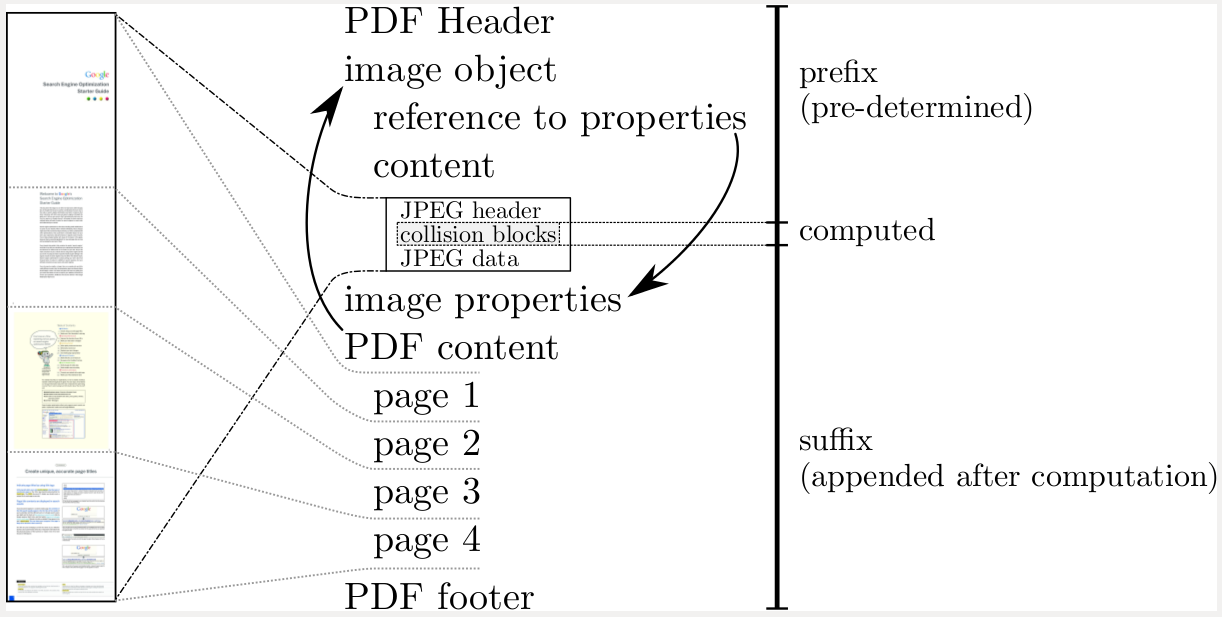
\includegraphics[width=0.8\textwidth]{img/2-img/pdf_format.png}
\end{center}

\end{frame}